\graphicspath{{chapters/01/images/}}
\chapter{Introduction}

\section{Introduction}

  \subsection{Cells}
  A cell is the basic unit of all known living organism.
  Different cell types have different roles which then organize to form higher levels of organization.
  The cell is a dynamical system whose behaviour is controlled and regulated by interaction between chemical species.

  \subsection{Biochemical reactions}
  The interactions between molecules in a cell are known are biochemical reactions.
  The chemical species in a cells are in constant movement and when they collide can cause a reaction if specific reaction conditions, like the activation energy, are satisfied.
  The outcome of a reaction is the consumption of some species and the production of new ones to help perform the necessary activities of the cell.

    \subsubsection{Reaction kinetics}
    The rate of a reaction is dependent on the species involved, the number of molecules present and a basal rate or affinity.
    The basal rate depends on the type and number of species involved and is often constant.
    The rates of reaction are determined by the reaction kinetics.

    \subsubsection{Pathways}
    Biochemical reactions are organized in pathways, a map showing the structural relationship of molecular species and their specific cellular response.
    They are involved in:

    \begin{multicols}{2}
      \begin{itemize}
        \item Metabolism.
        \item Signal transmission.
        \item Gene expression regulation.
      \end{itemize}
    \end{multicols}

    They are involved in different cellular purposes like:

    \begin{multicols}{2}
      \begin{itemize}
        \item Cell growth.
        \item Proliferation.
        \item Differentiation.
        \item Apoptosis.
      \end{itemize}
    \end{multicols}

    Explaining how a cellular function emerges from the molecular interactions needs a system-wide approach.

  \subsection{Systems biology}
  Systems biology is a new discipline that aims to understand how reactions give rise to specific cellular behaviours and a biological response.
  Its holistic view-point provide advantages in scientific and practical terms like:

  \begin{multicols}{2}
    \begin{itemize}
      \item Drug discovery.
      \item Disease mechanism explanation.
      \item Hypothesis verification.
    \end{itemize}
  \end{multicols}

    \subsubsection{Challenges of system biology}
    The challenges of systems biology are due to the large number of possible reactions and their non-linear dynamics.
    In these cases the stationary and time-invariant assumptions are often violated: the species constantly evolves according to changes in the cellular environments.
    Moreover some molecular species are present in low copy number or population.
    Reaction between these cause a significant fluctuation in their population, or biological noise, which may propagate along the pathway.

    \subsubsection{Stochasticity}
    The stochasticity in biochemical reaction can be also due to the fact that after many non-reactive collisions between species the biological system could choose a different cellular functioning.
    This is called multistability: a number of separated stable equilibria points are separated by unstable equilibria.
    Bistability is the simplest example of multistability, with only two stable equilibria.

  \subsection{Computational tools}
  Computational tools play a crucial role in systems biology.
  Introducing a model to represent the biological system's species of interest or states and the reaction between them or state transition, knowledge of the biology can be written in a formal form, often mathematically.

    \subsubsection{Biological models}
    A biological model is an abstraction of the system, but it is useful to understand it.
    A direct way to describe a model is to write down the list of reactions between species.
    Modelling a reaction network by coupled reactions is simple and flexible.

    \subsubsection{Computer simulation}
    Given a model, a computer simulation is used to realize its temporal evolution.
    The dynamical interactions between species can reveal indirect implications or unexpected behaviours.
    A simulation based experiment is called an in silico experiment.
    If results of this experiment agree with experimental data, they can be used to provide predictions for the dynamics of the system.

    \subsubsection{Advantages and applications of in silico experiment}
    With respect to traditional experiment, an in silico simulation has a number of advantages:

    \begin{multicols}{2}
      \begin{itemize}
        \item It takes less time.
        \item It is cheaper.
        \item They can detect indirect and hidden implications.
        \item It is possible to isolate vital genes from the cell, overcoming the necessity of maintaining a vital cell.
      \end{itemize}
    \end{multicols}

    The results of an in silico experiment are used to:

    \begin{multicols}{2}
      \begin{itemize}
        \item Test hypothesis.
        \item Suggesting new experiments.
      \end{itemize}
    \end{multicols}

    The predictive feature of computer simulations makes it useful to perform quantitative analysis.

  \subsection{Synthetic biology}
  Biological models and simulation contribute to the design and implementation of synthetic biology by providing a design focused experiment framework where models are reused as basic building blocks in a large model.
  This component-based model building is more effective and less error-prone than a traditional from-scratch approach.
  Moreover this component approach allows to reprogram cellular functions to serve for special purposes of biological research.

\section{Different levels of simulation}
To cope with the inherent multi-physics and multi-scale natures of biochemical reactions, different levels of simulation detail have been adopted to investigate their dynamical behaviour.

  \subsection{Molecular dynamics}
  Molecular dynamics deals with the microscopic level.
  In this type of simulation the structures, positions velocities and possible collisions of all molecules in the system are kept track of.
  Movement and reactions are governed by physical forces.
  A molecular dynamics simulation requires a very detailed knowledge of molecules in both time and space and requires a lot of computational power.
  Because of this it is used to simulate the system at the level of nanoscale of time and space.

  \subsection{Brownian dynamics}
  Brownian dynamics focuses on the dynamics of each individual species, skipping the molecular structure information and the weak long-range forces between species.
  The movement of a species is described as a random or Brownian walk among point-like structures.
  A reaction happens whenever the distance between two species is less than a predefined reaction radius.
  The time scale of a Brownian dynamics simulation is greatly improved over molecular dynamics, but it is still require too much computational power to deal with large scale models.

  \subsection{Deterministic simulation}
  A deterministic simulation is the highest coarse-grained approach which focuses on the macroscopic behaviour of biochemical reactions.
  Molecular species in the deterministic simulation approach are represented by their concentrations.
  The rate of change in the concentration of each species due to a reaction is directly proportional to the concentrations of the species involved in the reaction.
  The time evolution of a biochemical reaction network is described by a set of ordinary differential equations or ODEs.
  The deterministic simulation is fast, however its underlying assumption inherently oversimplifies biological reactions in which populations of molecular species are continuous variables and their changes due to single reaction firings are assumed to be negligible.
  The correctness of deterministic simulation is severely affected when stochasticity plays an important role in the dynamical behaviour of biochemical reactions.

  \subsection{Stochastic simulation}
  A stochastic simulation is a mesoscopic approach to provide a probabilistic description of the time evolution of biochemical reactions.
  It keeps track of a discrete count for the population, but abstracts all the detailed position and velocity information of each species.
  Each reaction in the network is assigned a non-negative chance to fire and to drive the system to a new state.
  The probability that a reaction occurs in a time interval is derived from the reaction kinetics.
  Each stochastic simulation step will select a reaction to fire according to its probability.

  \subsection{Problems with stochastic simulations}
  Although the stochastic simulation approach is faster than bot a molecular dynamics or Brownian dynamics approach, it is often computational demanding for simulating large biological systems.
  Moreover:

  \begin{itemize}
    \item Biochemical reactions, due to their multi-scale nature, are separated by different time scales in which some fast reactions will occur at rates greater than other reactions.
      The dynamical behaviour of biochemical reactions, after the short fluctuation time at the beginning, will be determined by the dynamics of the slow reactions.
      However, most of the time the simulation samples the fast reactions to realize the dynamics which is not the expected behaviour.
    \item The population of some species involved in reactions may be larger than others by many orders of magnitude.
      This implies that the fluctuations of some species are more or less significant when involving reactions fire.
    \item Keeping track of large population species is less efficient, since a coarse-grained simulation method can be applied without loss of total simulation accuracy.
      A model can combine and mix all of these aspects making the fast reactions occur frequently and drive the system very fast into a stable state.
    \item Due to the stochastic behaviour in a single simulation, many simulation runs must be performed to ensure a statistical accuracy and this requires a high computational effort.
      These issues raise a computational challenge for developing and implementing efficient stochastic simulation methods.
  \end{itemize}

\section{Network modeling}

[ missing lecture 2 ]

  \subsection{Logic models}
  Recap from the previous theory lecture: what is the main issue in using logic modelling with multiple levels? The update formulae need to be defined for each level, tricky extension procedure.

  \subsection{Petri nets}
  \textbf{Petri nets} are specific networks introduced in 1960s, with the idea to describe \emph{communication processes} (computer science field).
  We have two kinds of nodes:

  \begin{itemize}
    \item \textbf{\emph{places}}: container of entities
      \begin{itemize}
        \item \emph{tokens}: entities
      \end{itemize}
    \item \textbf{\emph{transitions}}: possibility to move one or more tokens to other places
  \end{itemize}

\noindent
  In order to model a chemical reaction, we can associate places to variables, transitions to chemical transformations and tokens to molecules.
  \\

  \begin{figure}[h!]
    \centering
    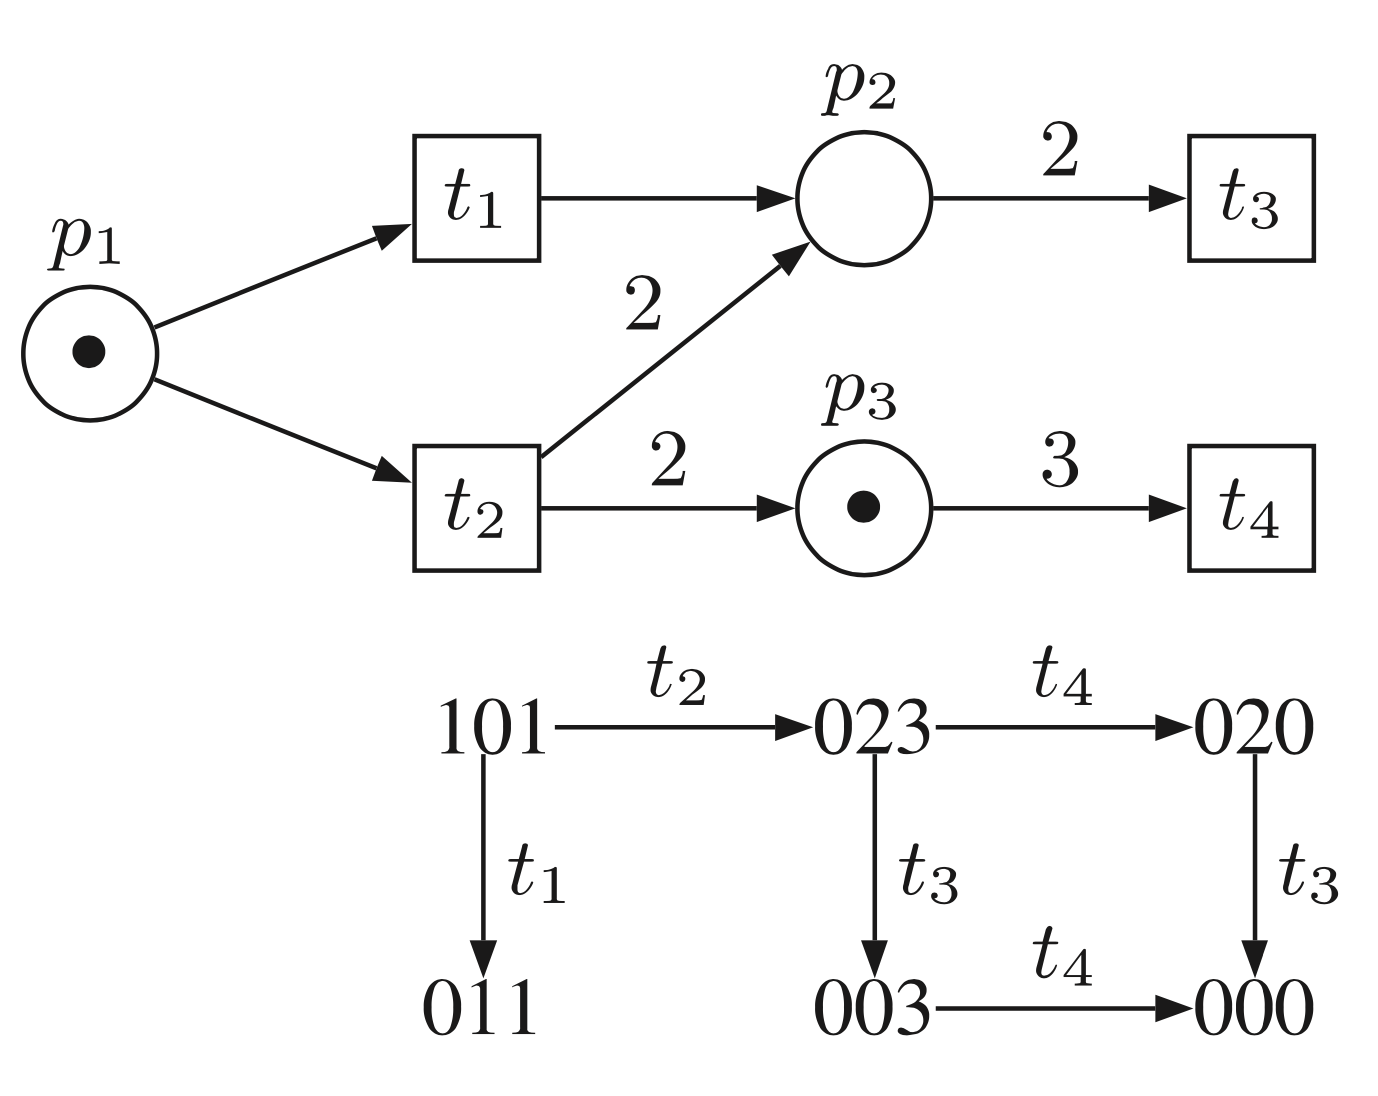
\includegraphics[width=0.5\textwidth]{petri_nets.png}
    \caption{PetriNets\_SimaoEtAl.pdf}
    \label{fig:petri}
  \end{figure}

\noindent
  Figure \ref{fig:petri}: in the example we have numbers inserted in places.
  The network will evolve according to the transitions applied.
  A transition can be \emph{enabled} or not to fire.
  E.g. there is one token in \(p_1\), so we know that \(t_1\) and \(t_2\) are enabled.
  Instead, \(t_4\) cannot be enabled, as 3 tokens are required but only one is present.
  \(t_2\) is taking the token from \(p_1\) and creating 2 tokens in \(p_2\) and \(p_3\); this allows to fire \(t_4\), since now \(p_3\) has the required number of tokens.

  \begin{enumerate}
    \def\labelenumi{(\alph{enumi})}
    \item shows the initial marking before firing the enable transition t;
    \item shows the marking after transition labeled reaction 1 fires.
      Places: hydrogen, oxygen and water.
      We can represent the stoichiometry of the reaction through the numbers on the edges and the numbers to the tokens.
    \end{enumerate}

  \begin{figure}
    \centering
    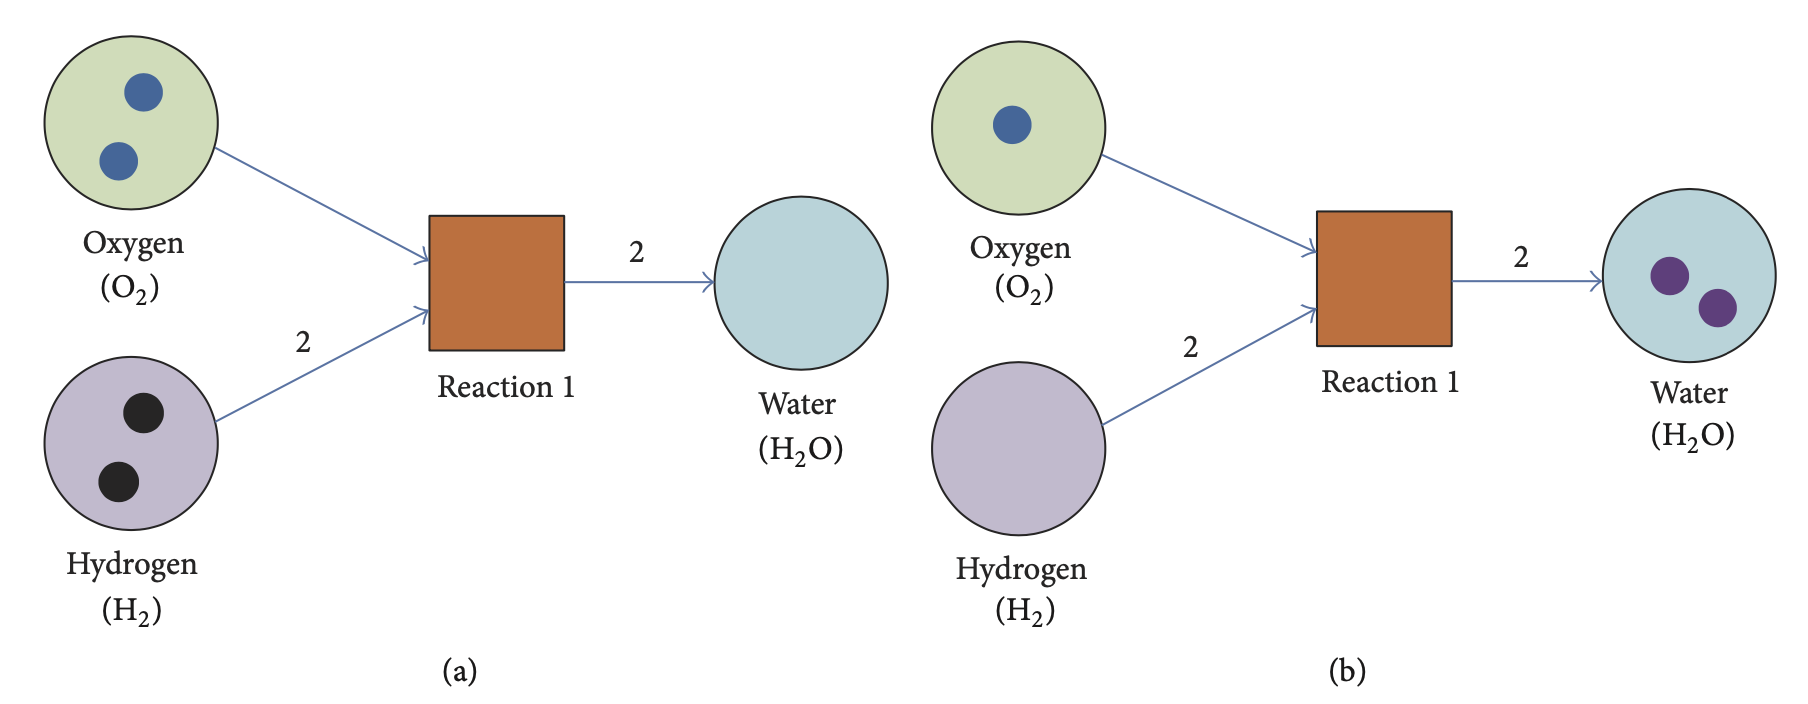
\includegraphics[width=0.7\textwidth]{/example_petri.png}
    \caption{Review\_ModelingComplexBiologicalSystems.pdf}
    \label{fig:expetri}
  \end{figure}

\noindent
  Figure \ref{fig:expetri}
  \begin{itemize}
  \item Pros: we have no constraint on the data type, not strictly boolean values. They allow to extend the number of items which can be associated to a model.
  \item Cons: there is no fixed rule for applying transitions. Furthermore, we are not encoding the reaction's complexity (all transitions are equally probable, but it is possible to weight the edges).
  \end{itemize}

  \noindent
  Having a dynamics based on the integers can be quite useful, as if we consider single chemical events we are working with discrete data.
  The exact stochastic algorithm works with integers.
  In differential equations instead we need real numbers.
  Also the discretization of the time step might not be a limitation, since time can be discretized in reality.
  The main limitation of network models is the \textbf{approximation of time},  as we are assuming that all the reactions take the same (unknown) amount of time.
  \\
  \\
  \noindent
 By upgrading the notation we can achieve more accurate representations:
  \begin{itemize}
    \item add inhibitory and test transitions.
    \item differentiate between discrete and continuous transitions.
  \end{itemize}

  \subsection{Rewriting systems}

    \subsubsection{P systems}
    Popular rewriting systems are \textbf{\emph{P systems}}, which are also called membrane systems.
    They are computational environments inspired to the structure of membranes.
    In particular, they define a hierarchy of membranes partitioning the space in different areas - similarly to a cell.
    In each region we can allocate entities and apply transformation rules.
    The rewriting rules change the value of each letter.
    The pedix \(_{in4}\) gives more details on the reaction.
    These kind of systems tend to use \emph{non-determinism}, they try to explore the full set of possibilities.

    \subsubsection{MP systems}
    The difference with standard P system is the association of functions to each reaction.
    In this way we can reconstruct the complexity of the reaction, since in the model we apply all possible reaction - which will produce an amount given by the function.

  \subsection{Equation-based approach}

    \subsubsection{ODE systems}
    Example: mass-action model
    \(A+E \underset{k_2}{\overset{k_1}{\rightleftharpoons}}A \mid E \stackrel{k_3}{\longrightarrow}B+E\)

  \subsection{Simulation algorithms}
  For simulating we need the specification of a stoichiometric matrix, a vector of integers (initial values) and a stochastic rate.
  \textbf{Exact simulation algorithms} are computationally intensive, but provide the most accurate solution.
  Stepwise, we will try to define faster strategies with the aim of compromising accurate dynamics and feasible solutions.
  It is also possible to rely on a mixture of technologies to focus on different results.
  If the well-mixed assumption is not fulfilled:

  \begin{itemize}
    \item partition the compartment in sub-compartments → approximation
    \item use more sophisticated algorithms
  \end{itemize}

  \noindent
  The \emph{stoichiometric matrix} tells us how the system evolves if one of the two functions is applied, but it is not enough for computing a simulation.
  There can be many reactions that arrive to the same definition of stoichiometric matrix.
  If we want to compute a dynamics we need to develop a series of states; at each step we require two ingredients:

  \begin{itemize}
    \item \(\tau\): tells how much later the system will evolve to another state
    \item \(\mu\): choose the reaction by considering the probability of execution of each reaction at the step
  \end{itemize}

\subsubsection{Reaction propensity}
  The reaction propensity is a function needed for the derivation of probability.
  The higher the propensity, the higher will be the strength of the reaction.
  Naturally, we will have a higher probability when a higher propensity is observed, but the two quantities are something different.
  The propensity is a property of the reaction, probability is a property of a reaction in the system (we need to take into account also other reactions) Instead of performing an in depth analysis of probability, we will choose a stochastic approach.
  It is only necessary to compute one evolution of the system per time.
